\subsection{Sistema de Observabilidad y Telemetría}\label{subsec:observabilidad}

La diversidad de flujos que componen Paralegales —síncronos y asíncronos, internos y dependientes de proveedores externos— exige un sistema transversal capaz de registrar, correlacionar y exponer el comportamiento del sistema en producción. Para atender esta necesidad, se conceptualizó e implementó un subsistema de observabilidad estructurada y telemetría que monitorea las integraciones de red con proveedores fundamentales, como los servicios de la Rama Judicial y la plataforma Samai del Consejo de Estado. El sistema opera de forma transversal, capturando eventos tanto en el BFF construido con Nuxt en el lado del servidor, como en la arquitectura de microservicios de \textit{backend} desplegados mediante AWS Lambda y programados en Go.

\subsubsection{Arquitectura e Implementación}

En arquitecturas de microservicios, una única acción desencadenada por el usuario puede atravesar múltiples componentes, redes y servicios distribuidos antes de retornar una respuesta. Esta naturaleza distribuida introduce complejidad al momento de diagnosticar fallos, identificar cuellos de botella o auditar interrupciones del servicio. Para abordar este desafío, la observabilidad se consolidó como un pilar arquitectónico del sistema, aprovechando la correlación de registros (\textit{logs}), métricas y trazas para deducir el estado interno del sistema a partir de sus salidas externas.

Para garantizar la consistencia de los datos de telemetría, el sistema evita la inyección manual y aislada de registros en cada punto de conexión. En su lugar, emplea el patrón de clientes HTTP interceptores (\textit{Intercepting HTTP Clients}) que generan telemetría unificada de forma transparente:

\begin{itemize}
  \item \textbf{Capa de \textit{backend} (Go):} se desarrolló una envoltura sobre el cliente HTTP nativo que emite eventos estructurados por cada salto de red (inicio de la petición, finalización o error). Mediante contextos del lenguaje (\texttt{context.WithValue}), se inyectan metadatos vitales a los registros de forma segura y propagada, tales como el nombre del servicio, el entorno de ejecución, la operación en curso y los identificadores de trazabilidad (ID de solicitud e ID de correlación).

  \item \textbf{Capa de \textit{frontend} (BFF en Nuxt):} se implementaron interceptores sobre la utilidad nativa de consumo de APIs. Mediante \textit{middlewares}, se extrae la información de la sesión del usuario para enriquecer la telemetría. Adicionalmente, se integraron mecanismos de saneamiento (\textit{sanitizers}) que garantizan que ninguna información confidencial —como contraseñas o \textit{tokens} de autorización— se filtre a los registros de texto.
\end{itemize}

Ambas capas convergen en un modelo de esquema estandarizado que emite eventos en formato JSON puro. Este sobre de datos unifica la estructura de los registros de toda la aplicación, eliminando ambigüedades y facilitando su indexación automática en la infraestructura de la nube.

\subsubsection{Infraestructura en la Nube y Monitoreo Proactivo}

El procesamiento y la visualización de la telemetría se encuentran completamente automatizados mediante Infraestructura como Código (IaC) a través de AWS CloudFormation. Esta infraestructura transforma los registros en bruto en conocimiento técnico accionable mediante cuatro mecanismos complementarios:

\begin{itemize}
  \item \textbf{Filtros de métricas deducidas:} el sistema analiza en tiempo real las cargas útiles JSON para derivar métricas operativas sin instrumentación de código adicional. Se capturan indicadores como el volumen total de tráfico (número de solicitudes), la tasa de errores de servidor (códigos HTTP 5xx) y las fluctuaciones en la latencia.

  \item \textbf{Alertas y matemáticas de métricas:} se configuraron alarmas agregadas que vigilan el comportamiento global de los microservicios. Mediante el análisis de percentiles (como el p95 para medir el peor caso de latencia) y sumatorias en ventanas de tiempo de cinco minutos, el sistema detecta degradaciones significativas del servicio de forma automática.

  \item \textbf{Notificaciones en tiempo real:} ante la activación de una anomalía, el sistema desencadena un flujo automatizado hacia un tópico SNS que invoca una función Lambda especializada. Esta función analiza las condiciones del fallo y transmite instantáneamente una notificación enriquecida al equipo de desarrollo a través de un canal de Telegram.

  \item \textbf{Panel de control centralizado:} la infraestructura despliega automáticamente un tablero de control (\textit{dashboard}) interactivo que consolida gráficos de series de tiempo y herramientas de análisis relacional (\textit{Logs Insights}), permitiendo ejecutar consultas estructuradas para identificar rápidamente la causa raíz de un error masivo.
\end{itemize}

La \autoref{fig:dashboard-observabilidad} muestra el panel de control de CloudWatch generado por la infraestructura, donde los gráficos de series de tiempo visualizan en tiempo real el volumen de peticiones, la tasa de errores y la distribución de latencias por servicio. La \autoref{fig:dashboard-observabilidad-alerts} complementa este panorama con la vista de alarmas configuradas, donde cada indicador refleja su estado actual —en alerta, en recuperación o saludable— de forma inmediatamente legible para el equipo de ingeniería.

\newcommand\dashboardObservabilidadCaption{Panel de control de CloudWatch con métricas de tráfico, errores y latencia de los microservicios. \hspace{1em}}
\begin{figure}[H]
  \centering
  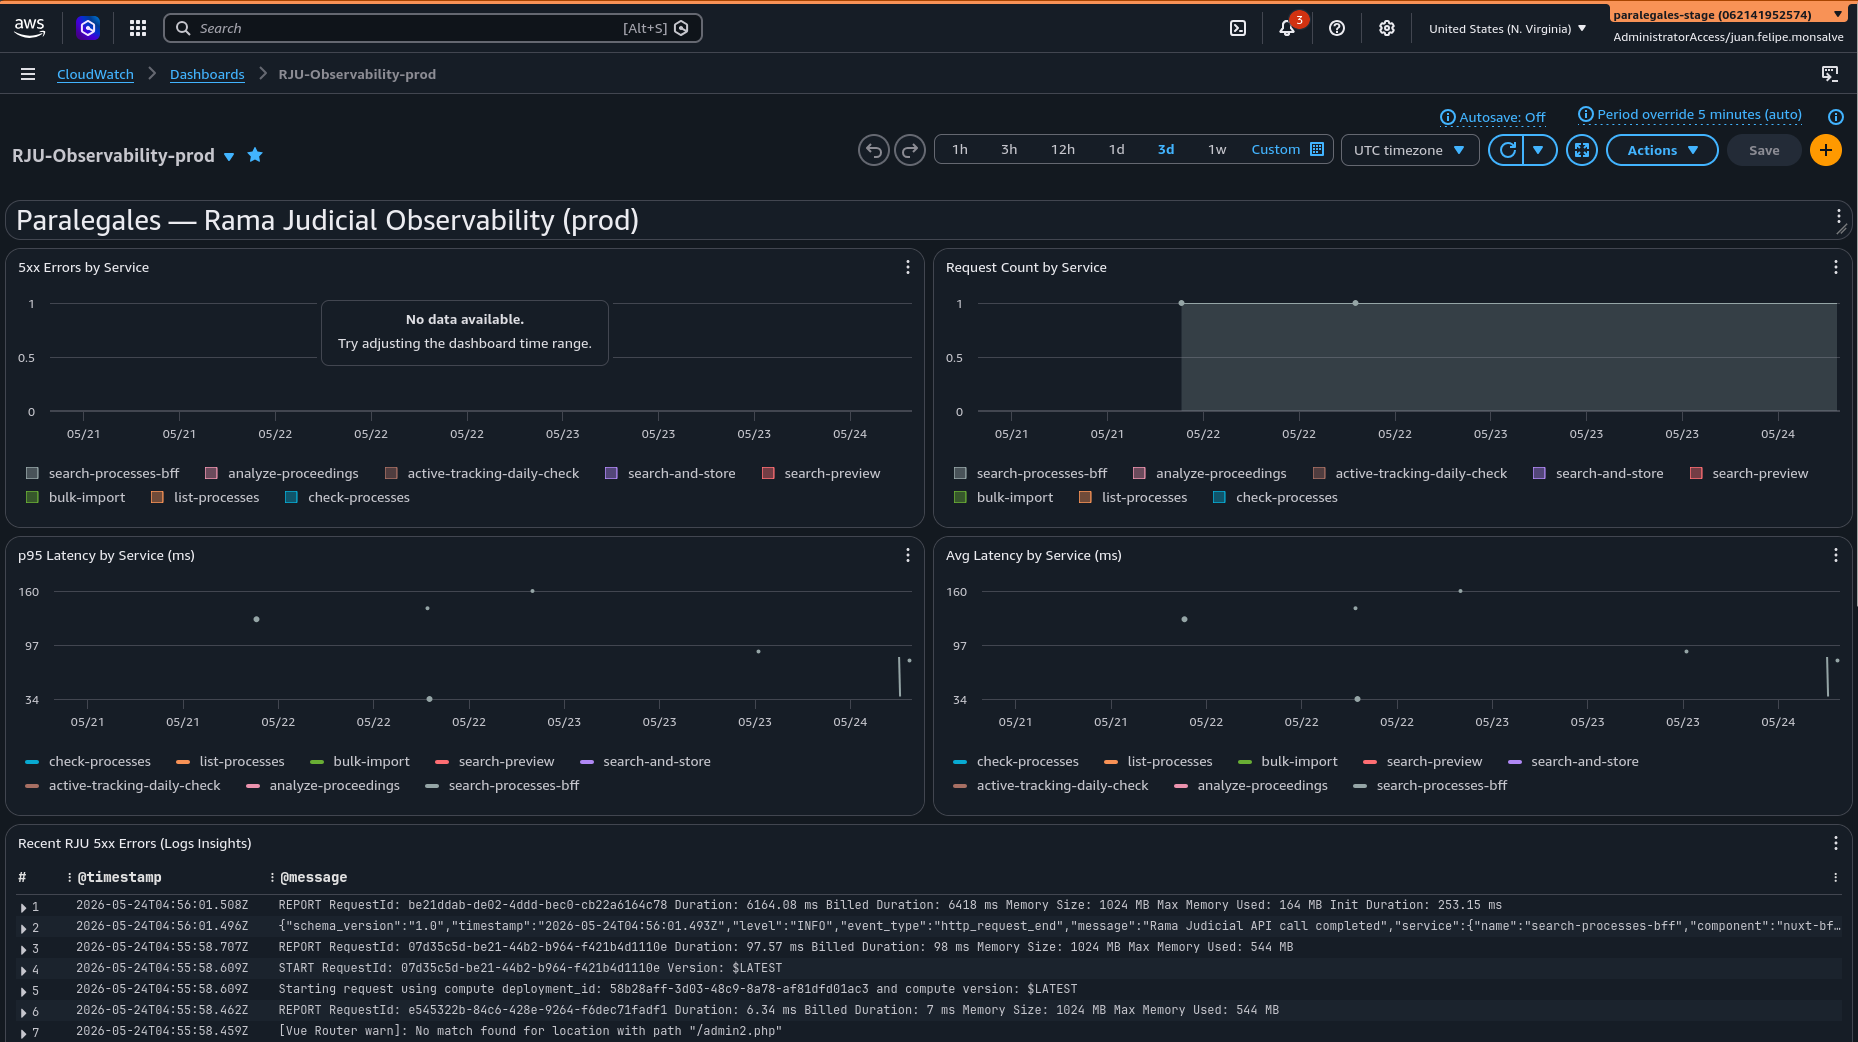
\includegraphics[width=1\textwidth]{img/figures/fig33-dashboard-observabilidad.png}
  \caption[\dashboardObservabilidadCaption]{\dashboardObservabilidadCaption Fuente: Elaboración propia.}
  \label{fig:dashboard-observabilidad}
\end{figure}

\newcommand\dashboardObservabilidadAlertsCaption{Vista de alarmas activas en CloudWatch con indicadores de estado por servicio monitoreado. \hspace{1em}}
\begin{figure}[H]
  \centering
  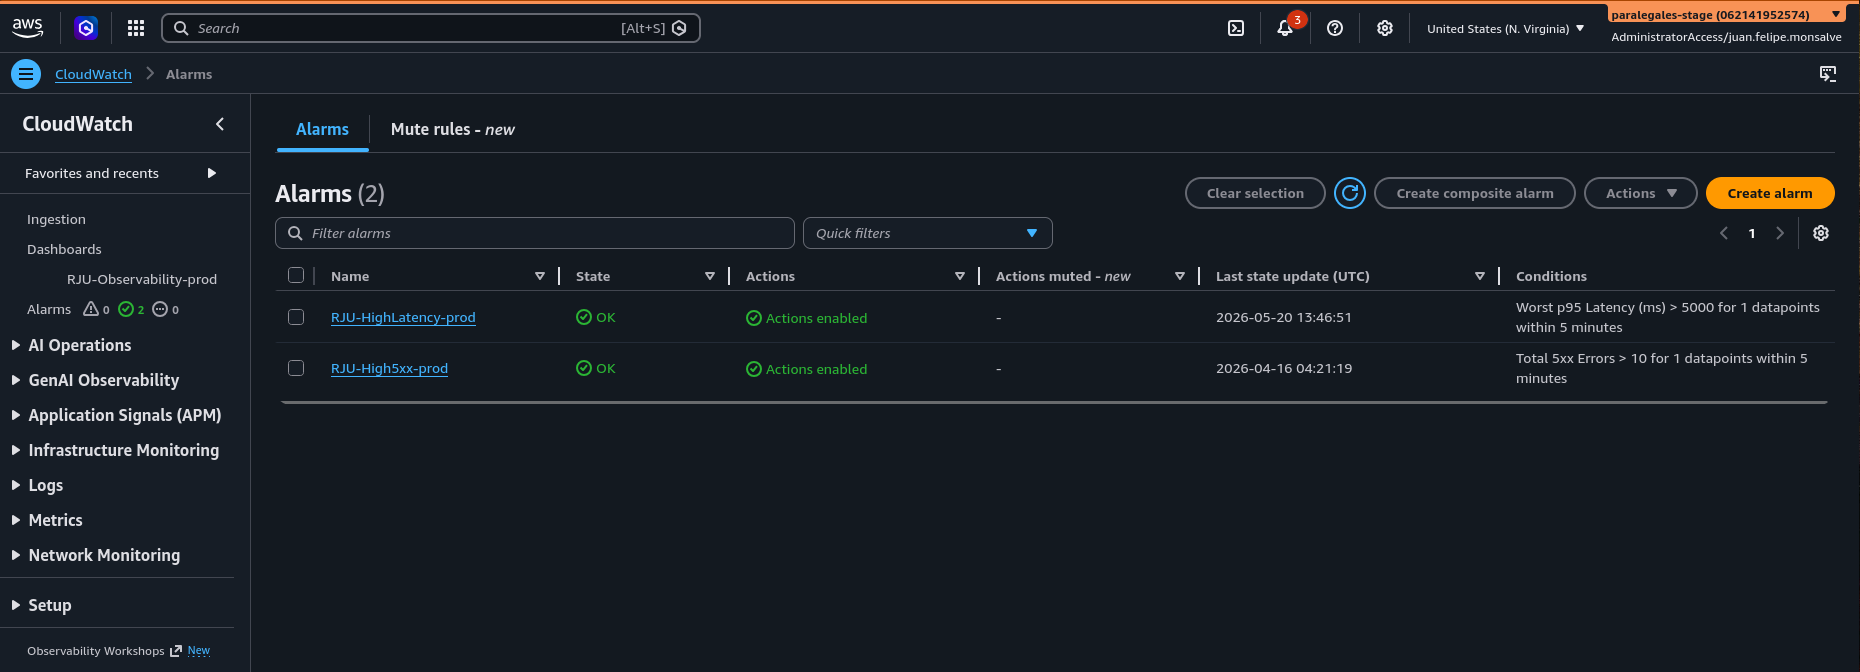
\includegraphics[width=1\textwidth]{img/figures/fig34-dashboard-observabilidad-alerts.png}
  \caption[\dashboardObservabilidadAlertsCaption]{\dashboardObservabilidadAlertsCaption Fuente: Elaboración propia.}
  \label{fig:dashboard-observabilidad-alerts}
\end{figure}

\newcommand\telegramAlertsObservabilityCaption{Canal de Telegram utilizado para la recepción de alertas automáticas del sistema. \hspace{1em}}
\begin{figure}[H]
  \centering
  \includegraphics[width=0.72\textwidth]{img/figures/fig13-telegram.png}
  \caption[\telegramAlertsObservabilityCaption]{\telegramAlertsObservabilityCaption Fuente: Elaboración propia.}
  \label{fig:telegram-alerts-observability}
\end{figure}

El impacto de este subsistema sobre la operación de la plataforma —la medición objetiva de la disponibilidad de los proveedores externos y la trazabilidad de errores por usuario— se valora como resultado del proyecto en el \autoref{subsec:resultado-c}.

Así como la observabilidad protege el sistema en su estado de operación continua, las prácticas que se describen a continuación resguardan la integridad y la calidad del código a lo largo de su proceso de evolución.
